\section{Hardware}

\begin{frame}
	\frametitle{Hardware}
	\framesubtitle{6 Node Specification}
	\begin{itemize}
		\item 1 x Login node
		\item 5 x Compute nodes
		\item 1 x Access point
		\item 1.8GHz Broadcom BC2711, Quad core Cortex-A72 (ARM v8 64 bit SoC)
		\item 4GB RAM
		\
	\end{itemize}
\end{frame}

\begin{frame}
	\frametitle{Hardware}
	\framesubtitle{Shopping List and Costs}
	\begin{table}[]
		\begin{tabular}{l|rcr}
			\hline
			\textbf{Item} & \textbf{Cost} & \textbf{Qty} & \textbf{Total} \\ \hline
			\textbf{Raspberry Pi 4B} & £34.00 & 7 & £204.00\\ 
			\textbf{PoE Hat} & £20.00 & 7 & £140.00\\ 
			\textbf{10 port switch with 8 x PoE} & £190.00 & 1 & £190.00\\
			\textbf{Patch cable - pack of 8} & £10.00 & 1 & £10.00\\
			\textbf{USB to SATA Adapter} & £9.00 & 1 & £9.00\\
			\textbf{120GB SATA SSD} & £10.00 & 1 & £10.00\\
			\textbf{80mm 5V USB fans - pack of 2} & £10.00 & 1 & £10.00\\
			\textbf{10" GeeekPi Rack} & £110.00 & 1 & £110.00\\
			
			\hline
			\textbf{Total} & & & £683.00\\
			\hline
		\end{tabular}
		\caption{Raspberry Pi 4B option}
		\label{tab:1}
	\end{table}
\end{frame}

\begin{frame}
	\frametitle{Hardware}
	\framesubtitle{The three stages of a miniHPC}
	
	\begin{figure}
		\centering
		\begin{subfigure}[b]{0.24\textwidth}
			\centering
			\includegraphics[width=\textwidth]{images/mini-HPC-proto1.png}
			\caption{Prototype 1}
			\label{fig:2.a}
		\end{subfigure}
		\hfill
		\begin{subfigure}[b]{0.24\textwidth}
			\centering
			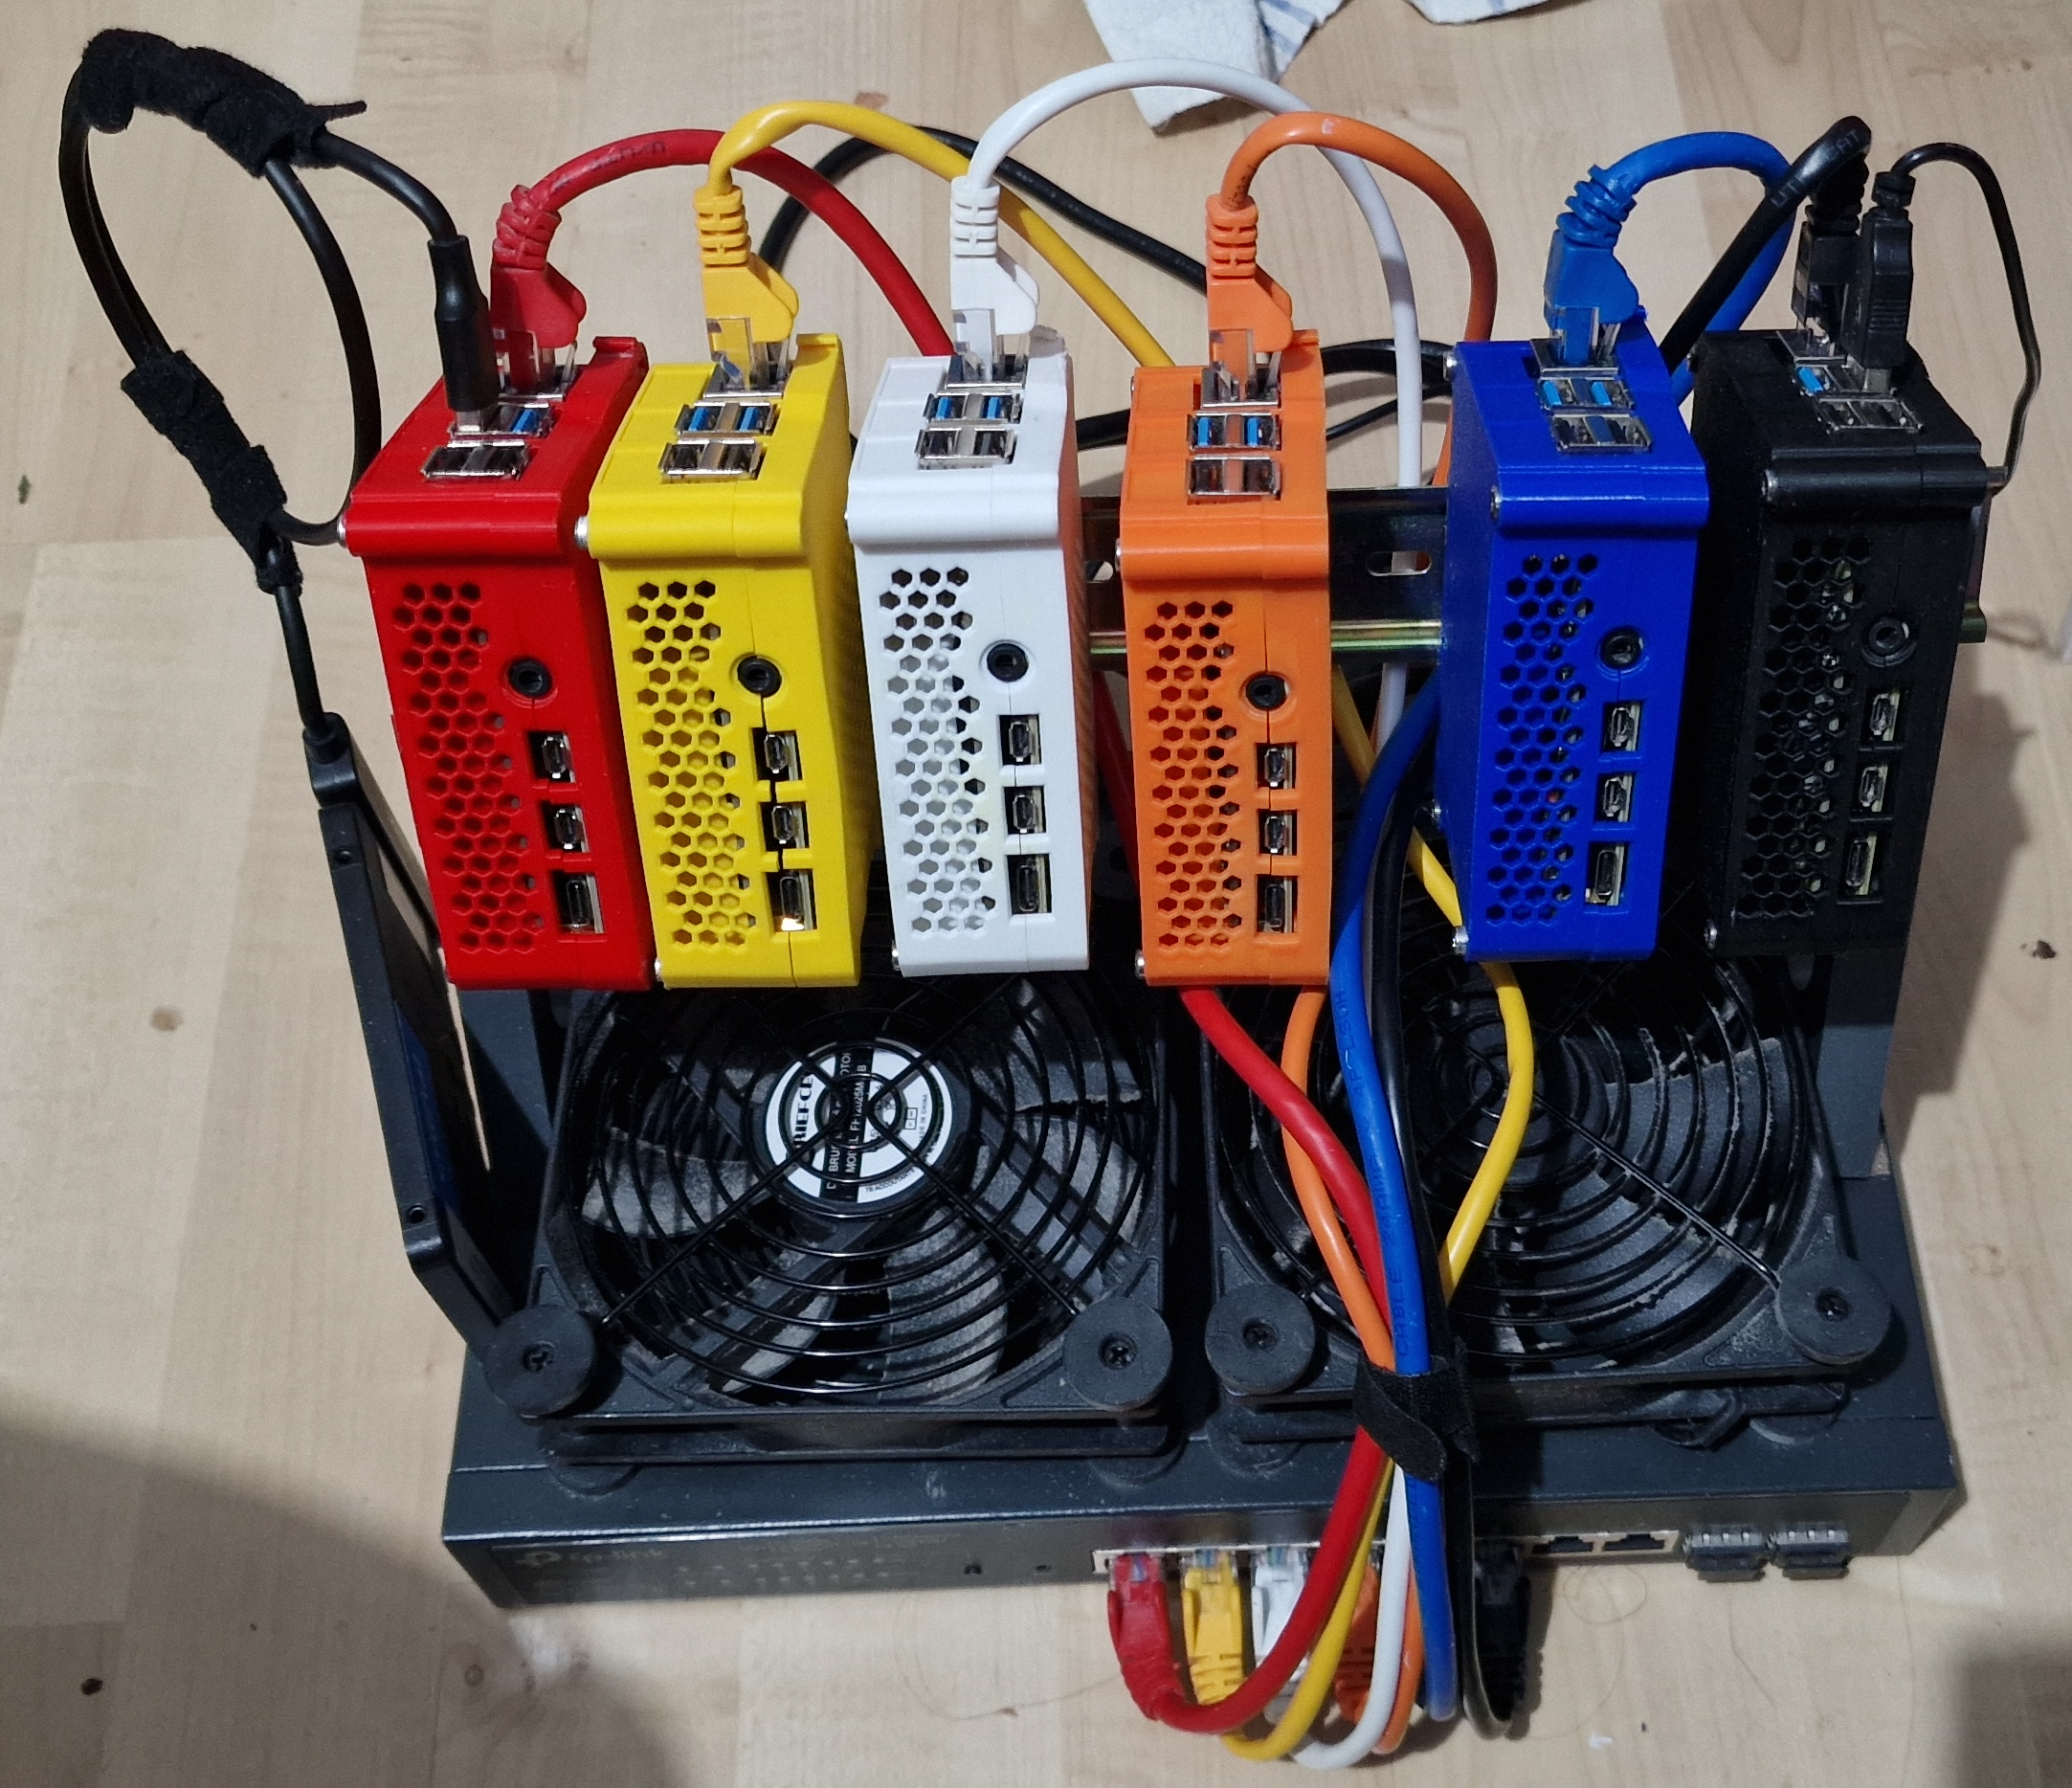
\includegraphics[width=\textwidth]{images/mini-HPC-proto2.png}
			\caption{Prototype 2}
			\label{fig:2.b}
		\end{subfigure}
		\hfill
		\begin{subfigure}[b]{0.24\textwidth}
			\centering
			\includegraphics[width=\textwidth]{images/mini-HPC-proto3.png}
			\caption{Prototype 3 front}
			\label{fig:2.c}
		\end{subfigure}
		\hfill
		\begin{subfigure}[b]{0.24\textwidth}
			\centering
			\includegraphics[width=\textwidth]{images/mini-HPC-proto3_back.png}
			\caption{Prototype 3 back}
			\label{fig:2.d}
		\end{subfigure}
		\caption{The Evolution of a miniHPC}
		\label{fig:2}
	\end{figure}
	
\end{frame}


